% REVIEW R3
% =============================================================================
% شکل‌های کیفی آزمایش چندمجموعه‌ای — خروجی tools/multidomain/make_qualitative_md_render.py
% نمونه قفل‌شده: thesis/figures/qualitative_md/manifest.json
% کسرهای افقی سرستون‌ها همان centres در thesis/figures/qualitative_md/geometry.json است.
% =============================================================================

% REVIEW R3
\begin{figure}[htbp]
  \centering
  \edaddbox{%
    \begin{tikzpicture}
      \node[anchor=south west, inner sep=0pt] (maps)
        {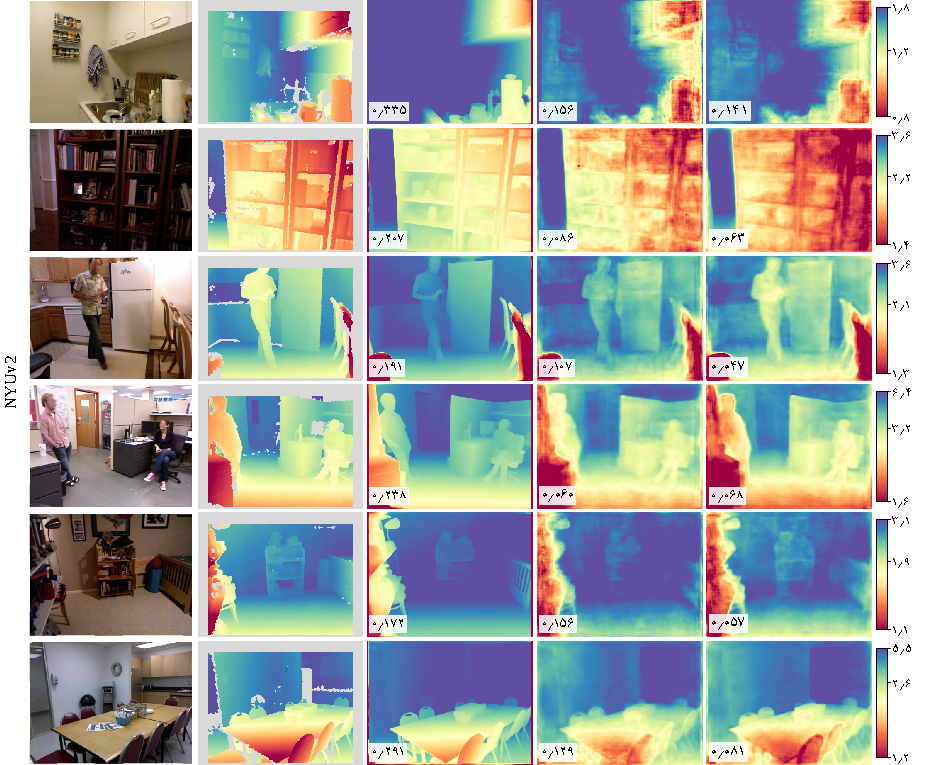
\includegraphics[width=\textwidth]{./figures/qualitative_md/qual_md_nyu.pdf}};
      \node[thnote, anchor=south, font=\scriptsize] at ([xshift=0.1192\textwidth]maps.north west) {\rl{تصویر ورودی}};
      \node[thnote, anchor=south, font=\scriptsize] at ([xshift=0.3016\textwidth]maps.north west) {\rl{عمق مرجع}};
      \node[thnote, anchor=south, font=\scriptsize, text=thBase] at ([xshift=0.4840\textwidth]maps.north west) {\rl{\tablepublishedmodel{}}};
      \node[thnote, anchor=south, font=\scriptsize, text=thControl] at ([xshift=0.6664\textwidth]maps.north west) {\rl{\tablecontrolmodel{}}};
      \node[thnote, anchor=south, font=\scriptsize, text=thProposed] at ([xshift=0.8488\textwidth]maps.north west) {\rl{\tableproposedmodel{}}};
    \end{tikzpicture}
    \caption[مقایسه کیفی سه مدل بر \lr{NYUv2}]{مقایسه کیفی سه مدل بر شش تصویر قفل‌شده از
    \lr{NYUv2}. نوار رنگ هر ردیف برحسب متر است و از عمق مرجع همان ردیف به دست آمده است.
    عدد هر خانه \lr{AbsRel} همان تصویر است و کمترین مقدار ردیف پررنگ شده است.
    \proposedmodel{} در پنج ردیف و \controlmodel{} در یک ردیف کمترین خطا را دارد.}
    \label{fig:qual_md_nyu}
  }
\end{figure}

% REVIEW R3
\begin{figure}[htbp]
  \centering
  \edaddbox{%
    \begin{tikzpicture}
      \node[anchor=south west, inner sep=0pt] (maps)
        {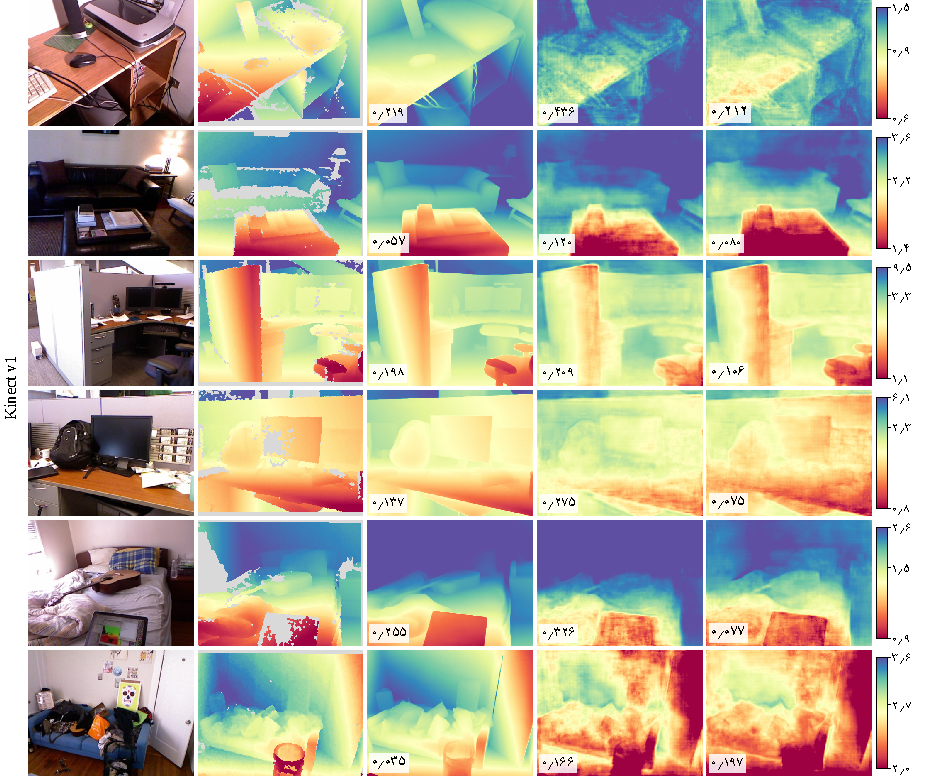
\includegraphics[width=\textwidth]{./figures/qualitative_md/qual_md_kv1.pdf}};
      \node[thnote, anchor=south, font=\scriptsize] at ([xshift=0.1192\textwidth]maps.north west) {\rl{تصویر ورودی}};
      \node[thnote, anchor=south, font=\scriptsize] at ([xshift=0.3016\textwidth]maps.north west) {\rl{عمق مرجع}};
      \node[thnote, anchor=south, font=\scriptsize, text=thBase] at ([xshift=0.4840\textwidth]maps.north west) {\rl{\tablepublishedmodel{}}};
      \node[thnote, anchor=south, font=\scriptsize, text=thControl] at ([xshift=0.6664\textwidth]maps.north west) {\rl{\tablecontrolmodel{}}};
      \node[thnote, anchor=south, font=\scriptsize, text=thProposed] at ([xshift=0.8488\textwidth]maps.north west) {\rl{\tableproposedmodel{}}};
    \end{tikzpicture}
    \caption[مقایسه کیفی سه مدل بر \lr{Kinect v1}]{مقایسه کیفی سه مدل بر شش تصویر قفل‌شده از
    داده‌های دیده‌نشده حسگر \lr{Kinect v1} در \lr{SUN RGB-D}، با قرارداد
    شکل~\ref{fig:qual_md_nyu}. \proposedmodel{} در چهار ردیف و \publishedbasemodel{} در دو ردیف
    کمترین خطا را دارد.}
    \label{fig:qual_md_kv1}
  }
\end{figure}

% REVIEW R3
\begin{figure}[htbp]
  \centering
  \edaddbox{%
    \begin{tikzpicture}
      \node[anchor=south west, inner sep=0pt] (maps)
        {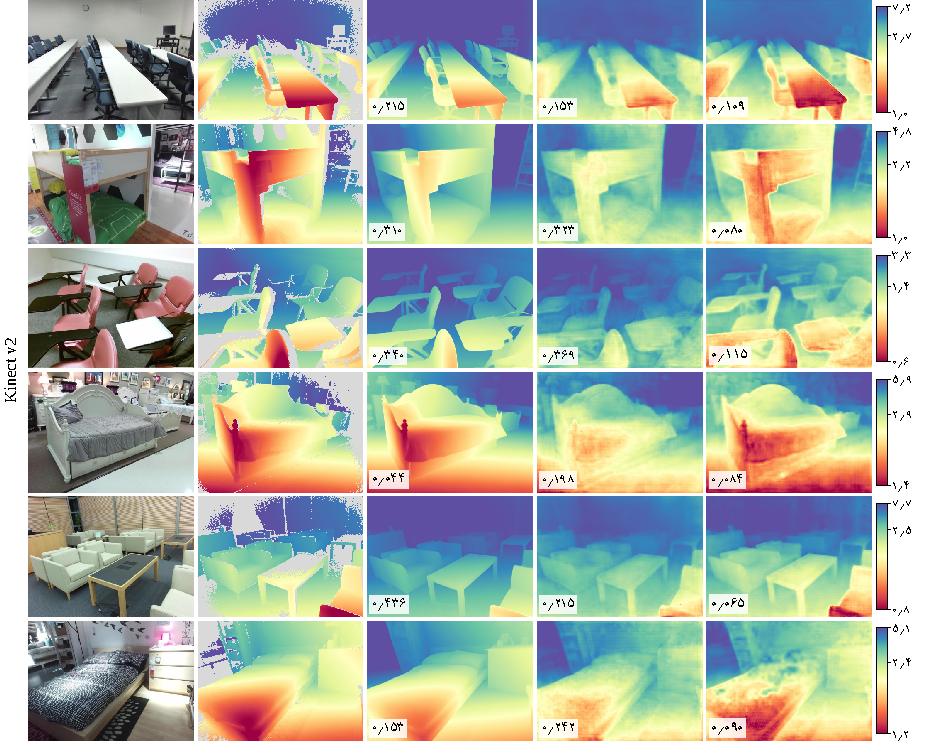
\includegraphics[width=\textwidth]{./figures/qualitative_md/qual_md_kv2.pdf}};
      \node[thnote, anchor=south, font=\scriptsize] at ([xshift=0.1192\textwidth]maps.north west) {\rl{تصویر ورودی}};
      \node[thnote, anchor=south, font=\scriptsize] at ([xshift=0.3016\textwidth]maps.north west) {\rl{عمق مرجع}};
      \node[thnote, anchor=south, font=\scriptsize, text=thBase] at ([xshift=0.4840\textwidth]maps.north west) {\rl{\tablepublishedmodel{}}};
      \node[thnote, anchor=south, font=\scriptsize, text=thControl] at ([xshift=0.6664\textwidth]maps.north west) {\rl{\tablecontrolmodel{}}};
      \node[thnote, anchor=south, font=\scriptsize, text=thProposed] at ([xshift=0.8488\textwidth]maps.north west) {\rl{\tableproposedmodel{}}};
    \end{tikzpicture}
    \caption[مقایسه کیفی سه مدل بر \lr{Kinect v2}]{مقایسه کیفی سه مدل بر شش تصویر قفل‌شده از
    داده‌های دیده‌نشده حسگر \lr{Kinect v2} در \lr{SUN RGB-D}، با قرارداد
    شکل~\ref{fig:qual_md_nyu}. \proposedmodel{} در پنج ردیف و \publishedbasemodel{} در یک ردیف
    کمترین خطا را دارد.}
    \label{fig:qual_md_kv2}
  }
\end{figure}

% REVIEW R3
\begin{figure}[htbp]
  \centering
  \edaddbox{%
    \begin{tikzpicture}
      \node[anchor=south west, inner sep=0pt] (maps)
        {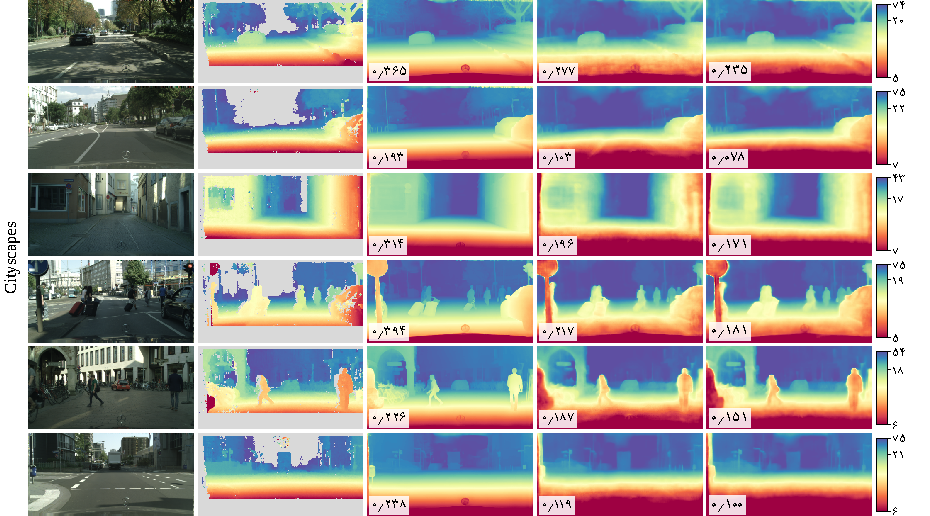
\includegraphics[width=\textwidth]{./figures/qualitative_md/qual_md_cityscapes.pdf}};
      \node[thnote, anchor=south, font=\scriptsize] at ([xshift=0.1192\textwidth]maps.north west) {\rl{تصویر ورودی}};
      \node[thnote, anchor=south, font=\scriptsize] at ([xshift=0.3016\textwidth]maps.north west) {\rl{عمق مرجع}};
      \node[thnote, anchor=south, font=\scriptsize, text=thBase] at ([xshift=0.4840\textwidth]maps.north west) {\rl{\tablepublishedmodel{}}};
      \node[thnote, anchor=south, font=\scriptsize, text=thControl] at ([xshift=0.6664\textwidth]maps.north west) {\rl{\tablecontrolmodel{}}};
      \node[thnote, anchor=south, font=\scriptsize, text=thProposed] at ([xshift=0.8488\textwidth]maps.north west) {\rl{\tableproposedmodel{}}};
    \end{tikzpicture}
    \caption[مقایسه کیفی سه مدل بر \lr{Cityscapes}]{مقایسه کیفی سه مدل بر شش تصویر قفل‌شده از
    \lr{Cityscapes}، با قرارداد شکل~\ref{fig:qual_md_nyu}. عمق مرجع این مجموعه از تناظر استریو
    به دست آمده و در بخش‌هایی از صحنه مقدار معتبر ندارد (خاکستری). \proposedmodel{} در هر شش
    ردیف کمترین خطا را دارد.}
    \label{fig:qual_md_cityscapes}
  }
\end{figure}

% REVIEW R3
\begin{figure}[htbp]
  \centering
  \edaddbox{%
    \begin{tikzpicture}
      \node[anchor=south west, inner sep=0pt] (maps)
        {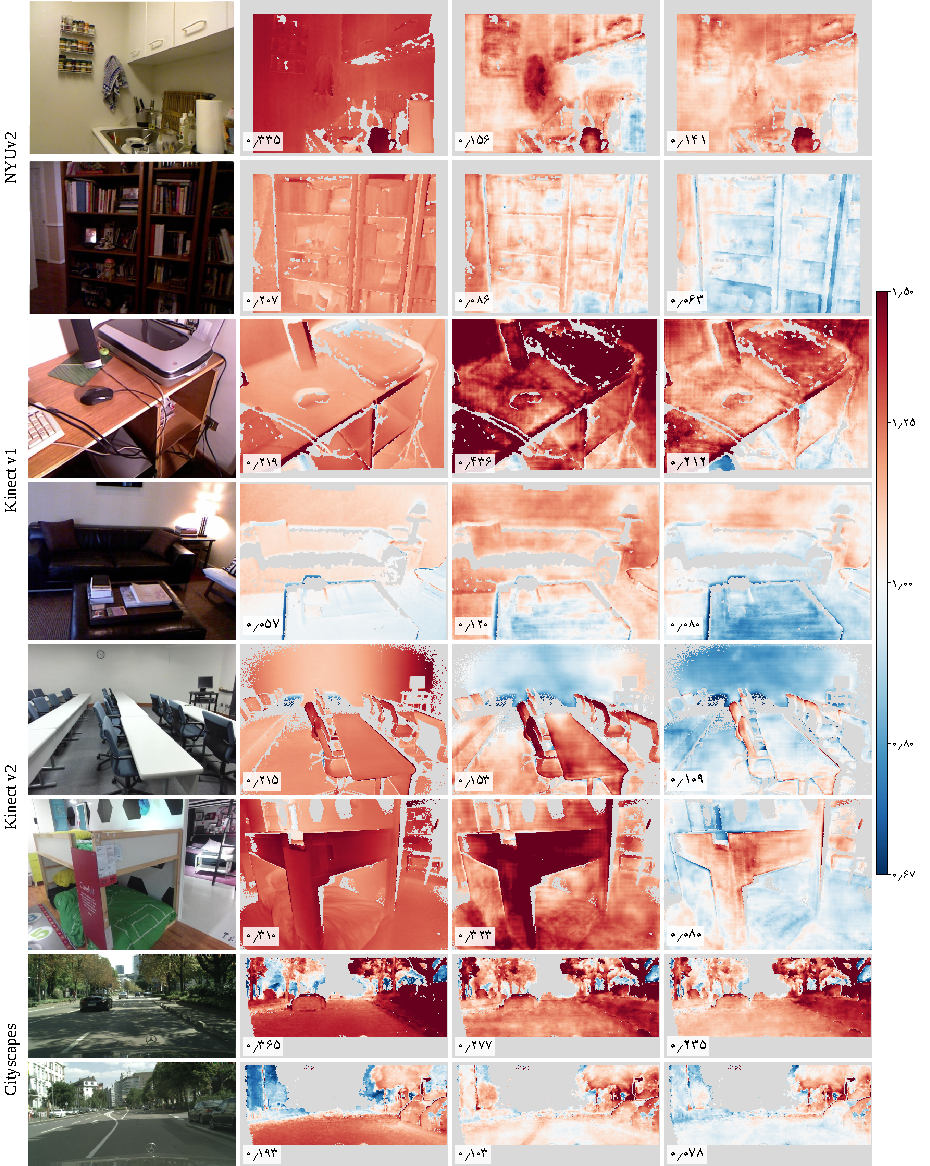
\includegraphics[width=0.80\textwidth]{./figures/qualitative_md/qual_md_error.pdf}};
      \node[thnote, anchor=south, font=\scriptsize] at ([xshift=0.1136\textwidth]maps.north west) {\rl{تصویر ورودی}};
      \node[thnote, anchor=south, font=\scriptsize, text=thBase] at ([xshift=0.2960\textwidth]maps.north west) {\rl{\tablepublishedmodel{}}};
      \node[thnote, anchor=south, font=\scriptsize, text=thControl] at ([xshift=0.4784\textwidth]maps.north west) {\rl{\tablecontrolmodel{}}};
      \node[thnote, anchor=south, font=\scriptsize, text=thProposed] at ([xshift=0.6608\textwidth]maps.north west) {\rl{\tableproposedmodel{}}};
    \end{tikzpicture}
    \caption[نقشه خطای علامت‌دار سه مدل]{نسبت عمق پیش‌بینی‌شده به عمق مرجع در پیکسل‌های معتبر،
    برای دو تصویر نخست هر مجموعه به ترتیب قفل‌شده. قرمز یعنی پیش‌بینی دورتر از مرجع، آبی یعنی
    نزدیک‌تر و سفید یعنی انطباق؛ نوار رنگ برای همه ردیف‌ها یکسان است. خاکستری پیکسل بدون
    عمق مرجع معتبر را نشان می‌دهد. عدد هر خانه \lr{AbsRel} همان تصویر است و کمترین مقدار ردیف
    پررنگ شده است؛ \proposedmodel{} در هفت ردیف و \publishedbasemodel{} در یک ردیف کمترین خطا را دارد.}
    \label{fig:qual_md_error}
  }
\end{figure}

% REVIEW R3
% REVIEW R20 (deleted: \edaddbox -> \eddelbox)
\begin{figure}[htbp]
  \centering
  \eddelbox{%
    \begin{tikzpicture}
      \node[anchor=south west, inner sep=0pt] (maps)
        {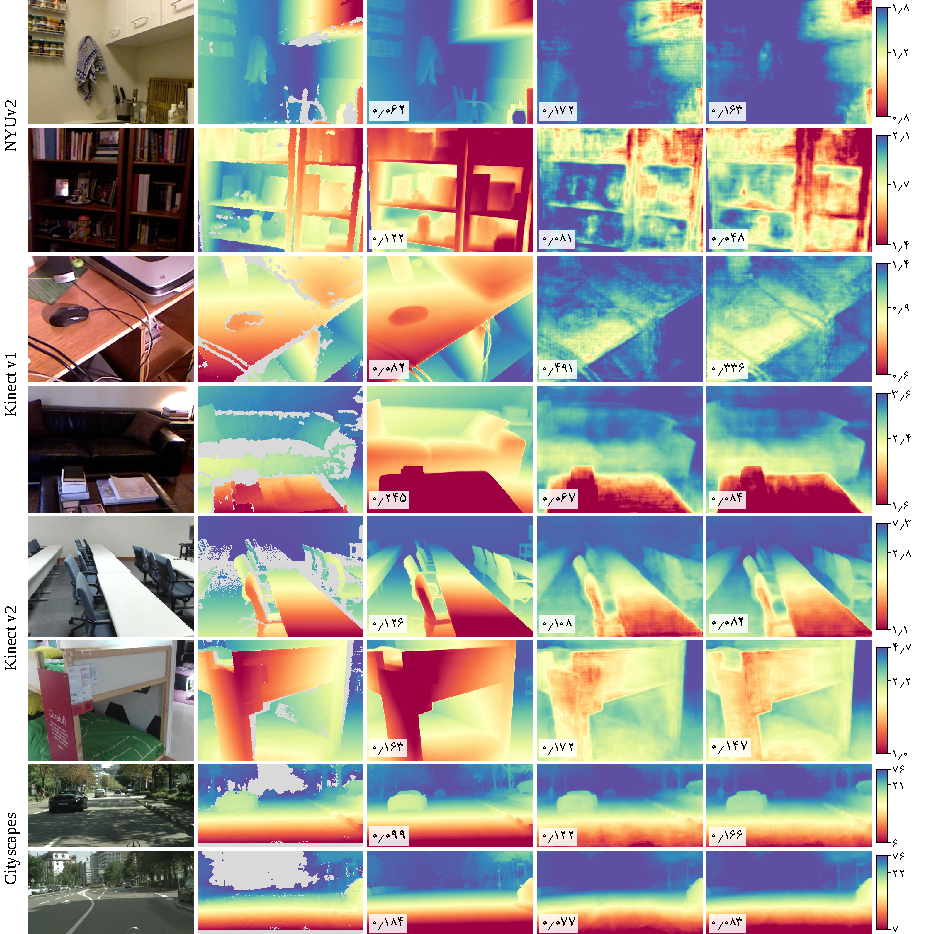
\includegraphics[width=0.88\textwidth]{./figures/qualitative_md/qual_md_shift.pdf}};
      \node[thnote, anchor=south, font=\scriptsize] at ([xshift=0.1049\textwidth]maps.north west) {\rl{تصویر ورودی}};
      \node[thnote, anchor=south, font=\scriptsize] at ([xshift=0.2654\textwidth]maps.north west) {\rl{عمق مرجع}};
      \node[thnote, anchor=south, font=\scriptsize, text=thBase] at ([xshift=0.4259\textwidth]maps.north west) {\rl{\tablepublishedmodel{}}};
      \node[thnote, anchor=south, font=\scriptsize, text=thControl] at ([xshift=0.5864\textwidth]maps.north west) {\rl{\tablecontrolmodel{}}};
      \node[thnote, anchor=south, font=\scriptsize, text=thProposed] at ([xshift=0.7469\textwidth]maps.north west) {\rl{\tableproposedmodel{}}};
    \end{tikzpicture}
    \caption[مقایسه کیفی در آزمون جابه‌جایی دوربین]{مقایسه کیفی در آزمون جابه‌جایی دوربین: برش
    مرکزی با ضریب \fadecimal{۱٫۵} از دو تصویر نخست هر مجموعه به ترتیب قفل‌شده، با قرارداد
    شکل~\ref{fig:qual_md_nyu}. در این ردیف‌ها \proposedmodel{} و \publishedbasemodel{} هر یک در
    سه ردیف و \controlmodel{} در دو ردیف کمترین خطا را دارند.}
    \label{fig:qual_md_shift}
  }
\end{figure}
